         \chapter{Wetenskapvaardighede}
    \setcounter{figure}{1}\setcounter{subfigure}{1}\label{m30853}
    \section{Inleiding}
            \nopagebreak
In die fisiese wetenskappe is daar baie vaardighede wat jy moet aanleer o.a. om met eenhede te werk, basiese wiskundige vaardighede en laboratoriumvaardighede. Hierdie hoofstuk hersien sommige van die vaardighede wat jy moet ken voordat jy kan begin om fisiese wetenskappe te leer. Hierdie hoofstuk is veronderstel om as  'n verwysingsgids te dien, wat jou help terwyl jy fisiese wetenskappe bestudeer. 
\section{Wiskundige vaardighede}
Jy moet wetenskaplike notasie verstaan en ook kan neerskryf. Jy moet ook maklik verskillende eenhede kan herlei en die onderwerp van  'n formule kan verander. Daarmee saam is konsepte soos tempo, direkte en omgekeerde eweredigheid, breuke en verhoudings asook die gebruik van die konstante in vergelykings, belangrik.  
\subsection*{Afronding}
Party getalle neem heeltemal te veel spasie en ink om neer te skryf. Dit is nie net onmoontlik om die getalle te skryf nie, maar om  'n getal met so baie desimale plekke neer te skryf is ongemaklik en gee selde  'n beter antwoord. Daarom skat ons eerder die getal tot  'n sekere hoeveelheid desimale plekke. \\
Om  'n desimale getal af te rond na  'n spesifieke hoeveelheid desimale plekke, is die vinnigste manier om  'n getal te skat. Byvoorbeeld: as jy $2,6525272$ tot drie desimale plekke wil afrond, tel jy drie plekke af na die desimaal. Daarna merk jy die punt met  'n voorstelling $|$: $2,652|5272$. Al die syfers regs van die $|$ word geïgnoreer nadat jy bepaal of die syfer wat in die derde desimaal staan opgerond of afgerond moet word. As die eerste getal na die $|$ groter as of gelyk aan 5 is, sal jy oprond (die syfer een meer maak), andersins rond jy af (los die getal soos hy is). Aangesien die eerste syfer na die $|$ 5 is, moet ons die syfer in die derde desimale plek oprond na  'n 3 en die finale antwoord van $2,6525272$ afgerond tot drie desimale plekke is $2,653$. \\
In 'n berekening met baie stappe, is dit die beste om die afronding tot reg aan die einde te laat. Dit verseker dat jou antwoord meer akkuraat is.
\subsection*{Wetenskaplike notasie}
In die wetenskap moet ons gereeld met baie groot of baie klein getalle werk. Hierdie getalle kan op  'n makliker (en meer kompakte) manier geskryf word in wetenskaplike notasie wat oor die algemeen as volg geskryf word:      
    \begin{equation*}
    N \times 10^{n}
      \end{equation*}
waar $N$  'n desimale getal tussen $0$ en $10$ voorstel, wat afgerond is tot  'n paar desimale plekke. $n$ staan bekend as die \textsl{eksponent} en is  'n integraal (heelgetal). As $n\greatthan{}0$ verteenwoordig dit hoeveel keer die desimale komma in $N$ na regs moet skuif. As $n\lessthan{}0$, verteenwoordig dit hoeveel keer die desimale komma in $N$ links moet skuif. Byvoorbeeld $3,24\ensuremath{\times}{10}^{3}$ verteenwoordig $3~240$ (die desimaal het 3 plekke na regs geskuif) en $3,24\ensuremath{\times}{10}^{-3}$ verteenwoordig $0,00324$ (die desimaal het 3 plekke na links geskuif).\\
Wanneer jy  'n getal in wetenskaplike notasie moet skryf moet jy eers uitwerk hoeveel keer die getal met 10 vermenigvuldig of deur 10 gedeel moet word sodat dit  'n getal tussen 1 en 10 vorm (m.a.w. die waarde van $n$) en wat die waarde van hierdie getal tussen 1 en 10 is (die waarde van $N$). Ons doen dit deur die aantal desimale plekke wat die komma skuif te tel.\\
Kyk na die volgende voorbeeld: skryf die spoed van lig ($299 ~792 ~458 \text{ m} \cdot \text{ s}^{-1}$) in wetenskaplike notasie tot twee desimale plekke. Ons moet eers kyk waar om die desimaal te sit as ons die getal tot twee desimale plekke moet skryf (m.a.w. vind die waarde van $N$) daarna tel ons die hoeveel plekke wat daar na die desimaal is om te bepaal wat die waarde van $n$ is.\\
In die voorbeeld moet die desimaal na die eerste $2$, geskryf word, maar aangesien die syfer na die $9$ 'n $7$ is, sal $N=3,00$. $n=8$ omdat daar $8$ syfers oor is na die desimale komma. Daarom sal die spoed van lig in wetenskaplike notasie, tot twee plekke na die desimaal, as volg lyk: $3,00 \times 10^{8} \text{ m} \cdot \text{s}^{-1}$. \\
Ons kan wetenskaplike notasie gebruik om optelling, aftrekking, vermenigvuldig en deel te doen. Die volgende twee uitgewerkte voorbeelde wys vir jou hoe om dit te doen.
\begin{wex}{Optelling en aftrekking met wetenskaplike notasie}
 {$1,99 \times 10^{-26} + 1,67 \times 10^{-27} - 2,79 \times 10^{-25} = ?$}
{\westep{Maak al die eksponente dieselfde}
Om getalle op te tel of af te trek in wetenskaplike notasie moet jy eers al die eksponente dieselfde maak: \\
$1,99 \times 10^{-26} = 0,199 \times 10^{-25}$ \\
$1,67 \times 10^{-27} = 0,0167 \times 10^{-25}$
\westep{Doen die bewerkings}
Wanneer die eksponente dieselfde is, kan ons eenvoudig die $N$ van elke getal optel of aftrek:\\
$0,199 + 0,0167 - 2,79 = -2,5743$ 
\westep{Skryf die finale antwoord neer}
Om die finale antwoord te kry moet ons die gemene eksponent weer terug sit:\\
$-2,5743 \times 10^{-25}$
}
\end{wex}
Let op dat ons dieselfde proses gebruik vir positiewe eksponente. Byvoorbeeld: $5,1 \times 10^{3} + 4,2 \times 10^{4} = 4,71 \times 10^{4}$. 
\begin{wex}{Vermenigvuldig en deel met wetenskaplike notasie}
 {$1,6 \times 10^{-19} \times 3,2 \times 10^{-19} \div 5 \times 10^{-21} $}
{ \westep{Vermenigvuldiging}
Wanneer ons vermenigvuldig of deel hoef die eksponente nie dieselfde te wees nie. Vir vermenigvuldiging tel ons die eksponente bymekaar en maal die $N$ terme:\\
$1,6 \times 10^{-19} \times 3,2 \times 10^{-19} = (1,6 \times 3,2) \times 10^{-19 + (-19)} = 5,12 \times 10^{-38}$
\westep{Doen deling}
Wanneer ons deel trek ons die eksponente af en deel die $N$ terme. As jy jou resultate van die vorige twee stappe gebruik, kry jy:\\
$2,56 \times 10^{-38} \div 5 \times 10^{-21} = (5,12 \div 5) \times 10^{-38 - (-19)} = 1,024 \times 10^{-18}$
\westep{Skyf die finale antwoord neer.}
Die antwoord is: $1,024 \times 10^{-18}$
}
\end{wex}
Let op dat ons dieselfde proses gebruik vir positiewe eksponente. Byvoorbeeld: $5,1 \times 10^{3} \times 4,2 \times 10^{4} = 21,42 \times 10^{7} = 2,142 \times 10^{8}$
\section{Eenhede}
Verbeel jou jy moet materiaal koop om gordyne te maak. Die winkelassistent moet weet hoeveel materiaal jy nodig het. Om net vir haar sê dat jy materiaal 2 wyd en 6 lank soek, is nie voldoende nie --- jy moet die \textbf{eenheid} ook spesifiseer (m.a.w. 2 \textsl{meter} wyd en 6 \textsl{meter} lank). Sonder die eenheid is die inligting onvolledig en sal die winkelassistent moet raai. As jy gordyne vir  'n pophuis wil maak sal die verhoudings dalk eerder 2 sentimeter wyd en 6 sentimeter lank wees!\\ 
Lengte is nie al wat eenhede het nie, alle fisiese hoeveelhede het eenhede (bv. tyd, temperatuur, afstand ens.)\\
\Definition{Fisiese hoeveelheid} { 'n Fisiese hoeveelheid is enige iets wat jy kan meet. So byvoorbeeld is lengte, temperatuur, afstand en tyd fisiese hoeveelhede.} 
Daar is verskillende sisteme van eenhede. Die hoof sisteme van eenhede is: 
\begin{itemize}
 \item SI-eenhede
\item c.g.s eenhede
\item Empiriese eenhede
\item Natuurlike eenhede
\end{itemize}
\subsection*{SI eenhede}
            \nopagebreak
Ons gaan deur die loop van die kursus SI-eenhede gebruik. SI-eenhede is eenhede waarop internasionaal ooreengekom is.
 \Definition{ SI eenhede } {Die naam \textsl{SI eenhede} kom van die Frans \textsl{Syst\`{e}me International d'Unit\'{e}s}, wat \textsl{internasionale sisteem van eenhede} beteken.  } 
Daar is sewe basiese SI-eenhede. Hulle word in tabel~\ref{tab:units:SIunits} gelys. Alle fisiese hoeveelhede het eenhede wat van hierdie sewe basiese eenhede afgelei kan word. Mens kan daarom een stel eenhede skep deur  'n ander stel basiese eenhede te definieer. \\
Die sewe eenhede word basiese eenhede genoem omdat nie een van hulle as kombinasies van die ander ses uitgedruk kan word nie. Hierdie basiese eenhede is soos die 26 letters van die alfabet. Mens kan baie verskillende woorde vorm deur verskillende kombinasies van die letters te gebruik.\par 
\begin{table}[H]
\centering
\begin{tabular}{|c|c|c|}\hline
\textbf{Basiese hoeveelheid} & \textbf{Naam} & \textbf{Simbool} \\
\hline lengte & meter & m\\ \hline 
massa & kilogram & kg\\ \hline 
tyd & sekonde & s\\ \hline 
elektriese stroom & ampere& A\\ \hline 
temperatuur & kelvin & K\\ \hline 
hoeveelheid stof & mol & mol\\ \hline 
ligintensiteit & kandela & cd\\ \hline
\end{tabular}
\caption{SI Basiese eenhede}\label{tab:units:SIunits}
\end{table}
 \subsection*{Die ander eenhede}
            \nopagebreak
Die SI-eenhede is nie die enigste eenhede wat gebruik word nie, maar dit word die meeste gebruik. In Wetenskap is daar drie ander stelle eenhede wat mens ook kan gebruik. Ons noem hulle bloot vir interessantheidshalwe. 
\begin{itemize}
 \item \textbf{c.g.s. Eenhede} \\
In die c.g.s-sisteem word meter vervang met sentimeter en kilogram met gram. Dit is  'n eenvoudige vervanging maar dit beteken dat alle eenhede wat van hierdie twee eenhede afgelei word, moet verander. Die eenhede vir krag en arbeid, byvoorbeeld, sal dus anders wees. Hierdie eenhede word meer gereeld in astrofisika en atoomfisika gevind.
\item \textbf{Empiriese eenhede} \\
Toe konings en koninginne destyds moes besluit watter eenhede hulle sou gebruik vir die lande, het empiriese eenhede die lig gesien. Alle basiese empiriese eenhede, behalwe wanneer jy tyd meet, is anders as SI-eenhede. Wanneer ons nie SI-eenhede gebruik nie, gebruik ons gewoonlik empiriese eenhede. Voorbeelde van empiriese eenhede is ponde, myle, gellings en tree. Hierdie eenhede word nogsteeds deur die Britte en Amerikaners gebruik. Jy kan jou voorstel dat die gebruik van verskillende eenhede in verskillende lande, problematies is vir wetenskaplike kommunikasie. Dit is juis hierom dat die eenhede waarop internasionaal ooreengekom is, eerder in gebruik geneem is.
\item \textbf{Natuurlike eenhede} \\
Hierdie is die mees gesofistikeerde eenhede. Wanneer jy hierdie eenhede gebruik word die mees fundamentele hoeveelhede (soos die spoed van lig) gelyk gemaak aan 1. Die beweegrede vir hierdie keuse is dat alle ander eenhede van die fundamentele eenhede behoort gebou te word. Die sisteem van eenhede word in hoogenergetiese fisika en kwantemeganika gebruik. 
\end{itemize}
% \subsection*{Writing units as words or symbols}
%             \nopagebreak
% Unit names are always written with a lowercase first letter, for example, we write metre and litre. The symbols or abbreviations of units are also written with lowercase initials, for example $m$ for metre and $\ell $ for litre. The exception to this rule is if the unit is named after a person, then the symbol is a capital letter. For example, the kelvin was named after Lord Kelvin and its symbol is K. If the abbreviation of the unit that is named after a person has two letters, the second letter is lowercase, for example Hz for hertz.\par 
\subsection*{Kombinasies van SI-eenhede}
            \nopagebreak
Om makliker met hierdie eenhede te kan werk, kry sommige kombinasies van basiese eenhede spesiale name. Dit is egter nooit verkeerd om alles tot basiese eenhede te reduseer nie. In tabel~\ref{tab:SIcombinations} word van die belangrikste kombinasies van basiese SI-eenhede, waaraan spesiale name toegeken is, gelys. Moenie bekommerd wees as van die formules op hierdie stadium onbekend lyk nie, ons gaan later in detail na hierdie (en nog baie ander) formules kyk. \\ 
Dit is baie belangrik dat jy in staat is om die eenhede korrek te herken. Byvoorbeeld: \textbf{newton} (N) is die ander naam vir \textbf{kilogram meter per sekonde kwadraat} (kg$\ensuremath{\cdot}$m$\ensuremath{\cdot}$s${}^{-2}$), terwyl \textbf{kilogram meter kwadraat per sekonde kwadraat} (kg$\ensuremath{\cdot}$m${}^{2}\ensuremath{\cdot}$s${}^{-2}$) as \textbf{joule} (J) bekend staan.
          \begin{table}[H]
        \begin{center}
\noindent
      \begin{tabular}{|l|l|l|l|}\hline
\textbf{Hoeveelheid} & \textbf{Formule} & \textbf{Eenhede uitgedruk in basiese eenhede}& \textbf{Naam van kombinasie} \\ \hline
Krag              & $ma$             & $\text{kg}\cdot \text{m} \cdot \text{s}^{-2}$      & N (newton)                   \\ \hline
Frekwensie         & $\frac{1}{T}$    & $\text{s}^{-1}$                                    & Hz (hertz)                   \\ \hline
Werk              & $Fs$             & $\text{kg} \cdot \text{m}^{2} \cdot \text{s}^{-2}$ & J (joule)                    \\ \hline
    \end{tabular}
\caption{Voorbeelde van kombinasies van SI basiese eenhede waaraan spesiale name toegeken is}
\label{tab:SIcombinations}
      \end{center}
\end{table}
    \par
\label{m30853*notfhsst!!!underscore!!!id306}
\subsection*{Voorvoegsels vir basiese eenhede}
            \nopagebreak
Jy kan nou getalle in wetenskaplike notasie skryf. Nog  'n belangrike aspek van eenhede is die voorvoegsels wat saam met  'n eenheid gebruik word. Voorvoegsels het  'n baie spesifieke gebruik as dit saam met eenhede gebruik word. Kilogram (kg) is  'n voorbeeld. 1 kg is gelyk aan 1 000 g of $1\ensuremath{\times}{10}^{3}$ g. Deur die ${10}^{3}$ en die g saam te groepeer kan ons dit vervang met die voorvoegsel k (kilo). Die k neem daarom die plek van die ${10}^{3}$. Die kilogram is die enigste basiese SI-eenheid wat  'n voorvoegsel kry. \\
In die wetenskap is alle voorvoegsels wat saam met eenhede gebruik word, magte van 10. Tabel~\ref{tab:unitprefixes} lys van hierdie voorvoegsels. Jy sal die meeste van hierdie voorvoegsels nie gebruik nie, maar jy moet die voorvoegsels wat vet gedruk is leer. Die kas (m.a.w. hoofletter of kleinletter) van die voorvoegsel se simbool is baie belangrik. As  'n letter twee keer in die tabel voorkom, word dit met hoofletters geskryf as die eksponente groter as een is en met kleinletters as dit kleiner as een is. So byvoorbeeld beteken M mega (10${}^{6}$) en m milli (10${}^{-3}$).

\Tip{Wanneer ons kombinasies van basiese SI-eenhede skryf sit ons  'n kolletjie ($\ensuremath{\cdot}$) tussen die eenhede om te wys dat verskillende basiese eenhede gebruik word. Die simbool vir meter per sekonde word, byvoorbeeld, eintlik as m$\ensuremath{\cdot}$s${}^{-1}$, geskryf en nie ms${}^{-1}$ of m/s nie. Alhoewel die laaste twee wel in toetse en eksamens aanvaar word, gaan ons net die eerste skryfwyse in hierdie boek gebruik.}

\begin{table}[H]
        \begin{center}
    \noindent
      \begin{tabular}{|l|l|l|l|l|l|}\hline
\textbf{Voorvoegsel} & \textbf{Simbool}  & \textbf{Eksponent} & \textbf{Voorvoegsel} & \textbf{Simbool} & \textbf{Eksponent} \\ \hline
yotta           & Y                & ${10}^{24}$       & yocto           & y               & ${10}^{-24}$      \\ \hline
zetta           &  Z               & ${10}^{21}$       &  zepto          & z               & ${10}^{-21}$      \\ \hline
eksa             &  E               & ${10}^{18}$       & atto            & a               & ${10}^{-18}$      \\ \hline
peta            & P                & ${10}^{15}$       & femto           & f               & ${10}^{-15}$      \\ \hline
tera            &  T               & ${10}^{12}$       &  piko           & p               & ${10}^{-12}$      \\ \hline
\textbf{giga}   & G                & ${10}^{9}$        & \textbf{nano}   & n               & ${10}^{-9}$       \\ \hline
\textbf{mega}   &  M               & ${10}^{6}$        & \textbf{mikro}  & $\mu $          & ${10}^{-6}$       \\ \hline
\textbf{kilo}   &  k               & ${10}^{3}$        & \textbf{milli}  & m               & ${10}^{-3}$       \\ \hline
\textbf{hekto}  &  h               & ${10}^{2}$        & \textbf{senti}  & c               & ${10}^{-2}$       \\ \hline
\textbf{deka}   &  da              & ${10}^{1}$        & \textbf{desi}   & d               & ${10}^{-1}$       \\ \hline
    \end{tabular}
\caption{Eenheid voorvoegsels}
      \end{center}
\label{tab:unitprefixes}
\end{table}
\Tip{Daar is nie spasies of kolletjies tussen die voorvoegsel en die simbool van die eenheid nie.}
Hier is  'n paar voorbeelde van hoe ons voorvoegsels gebruik:
\begin{itemize}[noitemsep]
  \item $40~000 \text{ m}$ kan as $40 \text{ km}$ (kilometer) geskryf word.
  \item $0,001 \text{ g}$ dieselfde as $1 \times{10}^{-3} \text{ g}$ en kan as $1 \text{ mg}$ (milligram) beskryf word.
  \item $2,5 \times {10}^{6}$ N kan as $2,5 \text{ MN}$ (meganewton) beskryf word.
  \item $250~000 \text{ A}$ kan as $250 \text{ kA}$ (kilo-ampere) or $0,250 \text{ MA}$ (mega-ampere) beskryf word.
  \item $0,000000075 \text{ s}$ kan as $75 \text{ ns}$ (nanosekondes) beskryf word.
  \item $3 \times{10}^{-7} \text{ mol}$ kan as $0,3 \times{10}^{-6} \text{ mol}$ beskryf word, wat dieselfde as $0,3 ~\mu \text{mol}$ (micromol)
\end{itemize}
\begin{exercises}{Scientific Notation }
            \nopagebreak \noindent
\begin{enumerate}[noitemsep, label=\textbf{\arabic*}. ] 
 \item Doen die volgende berekeninge:
    \begin{enumerate}[noitemsep, label=\textbf{\alph*}. ] 
     \item $1,63 \times 10^{5} + 4,32 \times 10^{6} - 8,53 \times 10^{5}$
     \item $7,43 \times 10^{3} \div 6,54 \times 10^{7} \times 3,33 \times 10^{5}$
     \item $6,21434534 \times 10^{-5} \times 3,2555 \times 10^{-3} + 6,3 \times 10^{-4}$
    \end{enumerate}
  \item Skryf die volgende in wetenskaplike notasie. Gebruik Tabel \ref{tab:unitprefixes} as verwysing.
    \begin{enumerate}[noitemsep, label=\textbf{\alph*}. ] 
      \item $0,511 \text{ MV}$
      \item $10 \text{ c}\ell $
      \item $0,5 ~\mu\text{m}$
      \item $250 \text{ nm}$
      \item $0,00035 \text{ hg}$
    \end{enumerate}
  \item Skryf die volgende eenhede neer deur die voorvoegsels in Tabel \ref{tab:unitprefixes} te gebruik.
    \begin{enumerate}[noitemsep, label=\textbf{\alph*}. ] 
      \item $1,602 \times{10}^{-19} \text{ C}$
      \item $1,992 \times{10}^{6} \text { J}$
      \item $5,98 \times{10}^{4} \text{ N}$
      \item $25 \times{10}^{-4} \text{ A}$
      \item $0,0075 \times{10}^{6} \text{ m}$
    \end{enumerate}
\end{enumerate}
\par \practiceinfo
 \par \begin{tabular}[h]{cccccc}
(1.) 02ed & (2.) 02c6  &  (3.) 02c7  & \end{tabular}
\end{exercises}
\subsection*{Die belangrikheid van Eenhede}
            \nopagebreak
Sonder eenhede sal baie wetenskaplikes se werk betekenisloos wees. Ons moet ons gedagtes duidelik uitdruk – eenhede gee betekenis aan die getalle wat ons meet en bereken. Afhangend van die eenheid wat ons gebruik, sal getalle verskil. As jy byvoorbeeld 12 water het, beteken dit niks nie. Jy kan 12 ml water of 12 liter water of selfs 12 bottels water hê. Eenhede is  'n belangrike deel van taalgebruik. Ons moet eenhede spesifiseer wanneer ons fisiese hoeveelhede uitdruk. Verbeel jou jy probeer  'n koek bak en die eenhede soos gram en milliliter, vir die melk, meel, suiker en bakpoeier is nie gespesifiseer nie.
\begin{groupdiscussion}{Belangrikheid van eenhede}
            \nopagebreak
Werk in groepe van 5 en bespreek die ander moontlike situasies waar eenhede wat verkeerdelik gebruik word tot jou nadeel of selfs gevaarlik kan wees. Kyk na voorbeelde by die huis, by die skool, in  'n hospitaal, as jy reis en in  'n winkel.
\end{groupdiscussion}
\begin{casestudy}{Die belangrikheid van eenhede}
            \nopagebreak
Lees die uittreksel van die CNN News, 30 September 1999 en beantwoord die vrae wat volg:\\
\textbf{NASA: Menslike fout veroorsaak verlies van Mars Wenteltuig 10 November, 1999}\\
Versuim om Britse mate na metrieke waardes te herlei het veroorsaak dat die Mars Klimaat Wenteltuig vernietig is.  'n Ondersoek, deur NASA van stapel gestuur, het Woensdag bevind dat die wenteltuig met  'n planeet gebots het voor dit  'n veilige wentelbaan kon bereik.\\
Die Mars Klimaat Wenteltuig,  'n sleuteltuig in die ruimte agentskap se verkenning van die rooi planeet, het op 23 September verdwyn na  'n 10 maande lange reis. Daar word vermoed dat die tuig gevaarlik naby aan die atmosfeer van Mars beweeg het, waar dit vermoedelik aan die brand geraak en in stukke gebreek het.\\
 'n Raad van ondersoek het bevind dat die NASA ingenieurs versuim het om die Britse mate van die vuurpyl se stootkrag na newton om te skakel, wat die metrieke sisteem is waarmee die krag van  'n vuurpyl gemeet word. Een Britse pond krag is gelyk aan 4, 45 newton.  'n Klein verskil tussen hierdie twee waardes kan veroorsaak dat die ruimtetuig te laag vlieg en hulle vermoed dat die tuig daarom in die planeet se atmosfeer vasgevlieg het en vernietig is.\\
Die ruimtetuig was  'n belangrike deel van die verkenning van die planeet. Van sy stasie op die rooi planeet, kon die Mars Klimaat Wenteltuig seine na die Mars Polar Lander stuur wat veronderstel is om volgende maand op Mars te land.\\
Die oorsaak van die verlies van die ruimtetuig is gewortel in  'n mislukte herleiding van Britse eenhede na metrieke eenhede en  'n segment van die navigasie-verwante sagteware van die ekspedisie wat op die grond gebaseer is.\\
\textbf{Vrae:}\\
\begin{enumerate}[noitemsep, label=\textbf{\arabic*}. ] 
\item Waarom het die Mars Klimaat Wenteltuig verongeluk. Antwoord in  jou eie woorde.
\item Hoe kon hierdie situasie vermy word?
\item Hoekom is die Mars Wenteltuig na Mars gestuur?
\item Dink jy dat verkenningsekspedisies in die ruimte belangrik is? Verduidelik jou antwoord.
\end{enumerate}
\end{casestudy}
\subsection*{Hoe om eenhede te herlei}
            \nopagebreak
Dit is baie belangrik dat jy weet dat daar verskillende sisteme van eenhede bestaan. Jy moet ook herleiding tussen die verskillende eenhede kan doen. As jy die eenhede kan verander (soos byvoorbeeld om millimeter na meter te herlei) kan dit jou baie help in die Wetenskap.\\ 
Die volgende herleidingsdiagramme sal jou help om van een eenheid na  'n ander te herlei.
\setcounter{subfigure}{0}
\begin{figure}[H]
\begin{center}
\scalebox{1} % Change this value to rescale the drawing.
{
\begin{pspicture}(0,-0.97605497)(5.9353123,0.976055)
\usefont{T1}{ptm}{m}{n}
\rput(0.27453125,-0.006054977){mm}
\usefont{T1}{ptm}{m}{n}
\rput(2.9545312,0.013945023){m}
\usefont{T1}{ptm}{m}{n}
\rput(5.664531,-0.006054977){km}
\psbezier[linewidth=0.04,arrowsize=0.05291667cm 2.0,arrowlength=1.4,arrowinset=0.4]{->}(0.296875,-0.15605497)(0.296875,-0.956055)(2.896875,-0.956055)(2.896875,-0.15605497)
\psbezier[linewidth=0.04,arrowsize=0.05291667cm 2.0,arrowlength=1.4,arrowinset=0.4]{->}(3.016875,-0.15605497)(3.016875,-0.956055)(5.616875,-0.956055)(5.616875,-0.15605497)
\usefont{T1}{ptm}{m}{n}
\rput(1.506875,-0.576055){\small $\div$1000}
\usefont{T1}{ptm}{m}{n}
\rput(4.326875,-0.576055){\small $\div$1000}
\usefont{T1}{ptm}{m}{n}
\rput(1.606875,0.50394505){\small $\times$1000}
\usefont{T1}{ptm}{m}{n}
\rput(4.346875,0.50394505){\small $\times$1000}
\psbezier[linewidth=0.04,arrowsize=0.05291667cm 2.0,arrowlength=1.4,arrowinset=0.4]{->}(2.896782,0.23767163)(2.9016154,0.92058134)(0.30180123,0.956055)(0.29696798,0.27314526)
\psbezier[linewidth=0.04,arrowsize=0.05291667cm 2.0,arrowlength=1.4,arrowinset=0.4]{->}(5.636782,0.23767163)(5.6416154,0.92058134)(3.0418012,0.956055)(3.036968,0.27314526)
\end{pspicture} 
}
\end{center}
\caption{Die afstand herleidingstabel}
\label{ch2:conversion1}
\end{figure}      
As jy eenhede van millimeter na meter wil herlei, moet jy deur  'n 1000 deel (volg die pyl van mm na m); of as jy van kilometer na millimeter wil herlei, moet jy vermenigvuldig met  'n 1000$\ensuremath{\times}$1000.\par 

Dieselfde metode kan gebruik word om milliliter na liter of kiloliter te verander. Gebruik figuur~\ref{ch2:conversion2} om volumes te herlei:
    \setcounter{subfigure}{0}
\begin{figure}[H] % horizontal\label{m30853*uid56}
\begin{center}
\scalebox{1} % Change this value to rescale the drawing.
{
\begin{pspicture}(0,-1.146055)(6.6696873,1.146055)
\usefont{T1}{ptm}{m}{n}
\rput(0.5271875,0.20394503){m$\ell$}
\usefont{T1}{ptm}{m}{n}
\rput(3.3912501,0.20394503){$\ell$}
\usefont{T1}{ptm}{m}{n}
\rput(6.1171875,0.20394503){k$\ell$}
\psbezier[linewidth=0.04,arrowsize=0.05291667cm 2.0,arrowlength=1.4,arrowinset=0.4]{->}(0.6784375,-0.326055)(0.6784375,-1.126055)(3.2784376,-1.126055)(3.2784376,-0.326055)
\psbezier[linewidth=0.04,arrowsize=0.05291667cm 2.0,arrowlength=1.4,arrowinset=0.4]{->}(3.3984375,-0.326055)(3.3984375,-1.126055)(5.9984374,-1.126055)(5.9984374,-0.326055)
\usefont{T1}{ptm}{m}{n}
\rput(1.9684376,-0.706055){\small $\div$1000}
\usefont{T1}{ptm}{m}{n}
\rput(4.6484375,-0.706055){\small $\div$1000}
\usefont{T1}{ptm}{m}{n}
\rput(1.9684376,0.673945){\small $\times$1000}
\usefont{T1}{ptm}{m}{n}
\rput(4.7084374,0.673945){\small $\times$1000}
\psbezier[linewidth=0.04,arrowsize=0.05291667cm 2.0,arrowlength=1.4,arrowinset=0.4]{->}(3.2783444,0.40767163)(3.2831779,1.0905813)(0.6833637,1.126055)(0.6785305,0.44314525)
\psbezier[linewidth=0.04,arrowsize=0.05291667cm 2.0,arrowlength=1.4,arrowinset=0.4]{->}(6.0183444,0.40767163)(6.0231776,1.0905813)(3.4233634,1.126055)(3.4185305,0.44314525)
\usefont{T1}{ptm}{m}{n}
\rput(3.3484375,-0.13605498){dm$^3$}
\usefont{T1}{ptm}{m}{n}
\rput(6.1471877,-0.116054974){m$^3$}
\usefont{T1}{ptm}{m}{n}
\rput(0.54265624,-0.13605498){cm$^3$}
\end{pspicture} 
}
\end{center}
\caption{Die volume herleidingstabel}
\label{ch2:conversion2}
 \end{figure}       
\begin{wex}{Herleiding 1}{Druk 3 800 mm in meter uit.}
 {
\westep{Gebruik die herleidingstabel} Gebruik Figuur~\ref{ch2:conversion1}. Millimeter is aan die linkerkant en meter in die middel.
\westep{Besluit in watter rigting jy beweeg} Jy  moet van mm na m gaan, so jy beweeg van links na regs.
\westep{Skryf die antwoord neer} $3 800 \text{ mm} \div 1~000 = 3,8 \text{ m}$ 
    }
\end{wex}
    \noindent
\nopagebreak
\begin{wex}{Herleiding 2}{Herlei 4,56 kg na g.}
{\westep{Soek die twee eenhede op die herleidingsdiagram}
Gebruik Figuur~\ref{ch2:conversion1}. Kilogram is dieselfde as kilometer en gram is dieselfde as meter.\\
\westep{Besluit in watter rigting jy beweeg}
Jy moet van kg na g gaan, so jy moet van regs na links beweeg.\\
\westep{Gebruik die diagram om te sien wat jy moet doen en skryf dan die antwoord neer}
$4,56 \text{ kg} \times 1~000 = 4~560 \text{ g}$}
\end{wex}
\subsubsection*{Nog twee nuttige herleidings}
            \nopagebreak
Ons moet gereeld in die wetenskap spoed en temperatuur herlei. Hierdie twee reëls sal jou help om dit te doen:
\begin{enumerate}[label=\textbf{\arabic*}.]
\item \textbf{Herleiding van spoed}\\
As jy $\text{km} \cdot \text{h}^{-1}$ herlei na $\text{m} \cdot \text{s}^{-1}$ moet jy met 'n $1~000$ maal en deur 'n $3~600$ (breuk) deel ($\dfrac{1000 \text{ m}}{3600 \text{ s}}$). Byvoorbeeld $72 \text{ km} \cdot \text{h}^{-1} \div 3,6 = 20 \text{ m}\cdot \text{s}^{-1}$.\\  
As jy $\text{m}\cdot \text{s}^{-1}$ herlei na $\text{km} \cdot \text{h}^{-1}$, moet jy met $3~600$ maal en deur $1~000$ deel ($\dfrac{3600 \text{ s}}{1000 \text{ m}}$). Byvoorbeeld $30 \text{ m}\cdot \text{s}^{-1} \times 3,6 = 108 \text{ km} \cdot \text{h}^{-1}$. 
\item \textbf{Herleiding van temperatuur}\\
Om van Kelvin na Celsius temperatuurskale te herlei is eenvoudig. Om van Kelvin na Celsius te herlei tel jy $273$. by. Om van Kelvin na Celsius te herlei moet jy $273$. aftrek. Die Kelvin temperatuur word deur ${T}_{K}$ en Celsius temperatuur word deur ${T}_{^{\circ}C}$ voorgestel:         
    \begin{equation*}
    {T}_{K}={T}_{^{\circ}C} + 273
      \end{equation*}
\end{enumerate}

\subsection*{Verander die onderwerp van die formule}
Jy moet gereeld in die wetenskap die onderwerp van  'n formule verander. Ons gaan na twee voorbeelde kyk. (Moenie bekommerd wees as jy nog nie weet wat die terme en simbole beteken nie, ons gaan later hierdie formules behandel).
\begin{enumerate}[label=\textbf{\arabic*}.]
 \item \textbf{Mol}\\
Die vergelyking om mol van molêre massa te bereken is: $n = \frac{m}{M}$, waar $n$ die aantal mol, $m$ die massa en $M$ die molêre massa is. Soos dit hier geskryf is, kan ons maklik die molêre massa van  'n stof kry. As ons egter die hoeveelheid mol het en die molêre massa wil bereken, moet ons eers die formule verander. Jy sal sien dat ons eenvoudig aan albei kante van die vergelyking met die molêre massa kan vermenigvuldig en dan aan albei kante deur die hoeveelheid mol kan deel:
\begin{eqnarray*}
 n & = & \frac{m}{M} \\
nM & = & m \\
M & = & \frac{m}{n}
\end{eqnarray*}
As ons nou die massa soek, kan ons $m = nM$ gebruik.
\item \texbf{Energie van  'n foton of ligkwantum}\\
Die vergelyking vir die energie van  'n foton is $E = h\frac{c}{\lambda}$, waar $E$ energie, $h$ Planck se konstante, $c$ spoed van lig en $\lambda$ golflengte is. Om $c$ te bereken moet ons die volgende doen:
\begin{eqnarray*}
 E & = & h\frac{c}{\lambda} \\
E \lambda & = & hc \\
c & = & \frac{E \lambda}{h}
\end{eqnarray*}  
Net so kan ons die golflengte kry deur $\lambda = \frac{hc}{E}$ te gebruik en Planck se konstante deur $h =  \frac{E \lambda}{c}$ te gebruik.
\end{enumerate}
\subsection*{Tempo, eweredigheid en verhouding}
In die wetenskap wil ons dikwels weet hoe  'n hoeveelheid vergelyk met  'n ander hoeveelheid of hoe een ding verander oor die loop van tyd. Om dit te doen moet ons tempo, eweredigheid en verhouding verstaan. \\
\textbf{Tempo:}\\
Die tempo waarteen iets gebeur is die hoeveelheid keer wat dit oor  'n sekere tydperk gebeur. Die tempo van iets is altyd  'n verandering per eenheid tyd. Daarom kan ons die tempo van die verandering van snelheid per eenheid tyd ($\frac{\Delta \vec{v}}{t}$) of die tempo van die verandering in die konsentrasie per eenheid tyd ($\frac{\Delta{C}}{t}$). (Let op dat $\Delta$  'n verandering aandui). \\
\textbf{Verhouding en breuke:}\\
 'n Breuk is  'n getal wat deur sy dele verteenwoordig word en word as volg geskryf: $\frac{a}{b}$, waar $a$ die teller en $b$ die noemer is.  'n Verhouding sê vir ons die relatiewe grootte van  'n hoeveelheid (bv. die hoeveelheid mol van die reagens) vergelyk met  'n ander hoeveelheid (bv. die hoeveelheid mol van die produk): $2:1$, $4:3$, ens. Verhoudings kan ook as breuke en persentasies (breuke met  'n noemer van 100) geskryf word.\\
\textbf{Eweredigheid:}\\
Eweredigheid is hoe  'n mens die verhouding tussen twee waardes of twee konstante beskryf. Ons kan sê dat $x$ eweredig is aan $y$ ($x \propto y$), of dat $a$ omgekeerd eweredig aan $b$ ($a \propto \frac{1}{b}$) is. Dit is belangrik om die verskil tussen direkte en omgekeerde eweredigheid te verstaan.
\begin{itemize}
 \item \textbf{Direkte eweredigheid}\\
Twee waardes of konstante is direk eweredig as 'n verandering in die een lei tot dieselfde soort (groter of kleiner) verandering in die ander een. Dit is  'n meer-meer verhouding. Ons kan dit voorstel as $y \propto x$ of $y = kx$ waar $k$ die eweredigheidskonstante is. Ons moet $k$ insluit aangesien ons nie weet met hoeveel $x$ verander wanneer $y$ verander nie. $x$ kan met 2 verander vir elke 1 in $y$. As ons die twee direk eweredige veranderlikes op  'n grafiek uitstip, kry ons  'n reguit lyn wat deur die oorsprong gaan $(0;0)$:
\\
\scalebox{.6}{
\begin{pspicture}(0,0)(6,6)
\psaxes[linewidth=1pt,labels=none,ticks=none]{->}(0,0)(0,0)(5,5)
\psplot[plotpoints=200]{0}{5}{x}
\end{pspicture}}
 
\item \textbf{Omgekeerde eweredigheid}\\
Twee waardes of konstante is omgekeerd eweredig aan mekaar as  'n verandering in die een lei tot die teenoorgestelde verandering in die ander een. Ons kan dit voorstel as $y = \frac{k}{x}$. Hierdie is  'n meer-minder verhouding. As ons die twee omgekeerd eweredige veranderlikes op  'n grafiek uitstip kry ons  'n kurwe wat nooit die as kruis nie ( 'n hiperbool).\\
\scalebox{.7} % Change this value to rescale the drawing.
{
\begin{pspicture}(0,-2.8429167)(5.7458334,2.8629167)
\rput(0.74583334,-2.1570833){\psaxes[linewidth=1pt,labels=none,ticks=none]{->}(0,0)(0,0)(5,5)}
\psbezier[linewidth=0.04](0.92583334,2.8429167)(1.1658334,-0.41708332)(0.54583335,-1.8970833)(5.7258334,-1.9770833)
\end{pspicture} 
}
\end{itemize}

\subsection*{Die konstante in vergelykings}
 'n Konstante in  'n vergelyking het \textbf{altyd} dieselfde waarde. Byvoorbeeld in die vergelyking vir die spoed van lig is ($c = 2,99 \times 10^{8} \text{ m} \cdot \text{ s}^{-1}$), Planck se konstante ($h$) en Avogadro se nommer ($N_A$) almal voorbeelde van konstante waardes wat in die wetenskap gebruik word. Die volgende tabel lys al dit konstante waardes wat jy in die boek gaan teëkom.
\begin{table}[H]
 \begin{center}
  \begin{tabular}{|l|l|l|l|}\hline
   \textbf{Konstante} & Simbool & \textbf{Waarde en eenhede} & \textbf{SI Eenhede} \\ \hline
Atomiese massa-eenheid & $u$ & $1,67 \times 10^{-24} \text{ g}$ & $1,67 \times 10^{-27} \text{ kg}$ \\ \hline
Lading op 'n elektron & $e$ & $-1,6 \times 10^{-19} \text{ C}$ & $-1,6 \times 10^{-19} \text{ s}\cdot \text{A}$ \\ \hline
Spoed van klank (in lug, at $25^{\circ}$) & & \multicolumn{2}{l|}{$344 m \cdot s^{-1}$} \\ \hline
Spoed van ligh & $c$ & \multicolumn{2}{l|}{$3 \times 10^{8} m \cdot s^{-1}$} \\ \hline
Planck se konstante & $h$ & $6,626 \times 10^{-34} \text{ J} \cdot \text{s}$ & $6,626 \times 10^{-34} \text{ kg} \cdot \text{m}^{2} \text{s}^{-1}$ \\ \hline
Avogadro se getal & $N_{A}$ & \multicolumn{2}{l|}{$6,022 \times 10^{23}$} \\ \hline
Gravitasie-versnelling & $g$ & \multicolumn{2}{l|}{$9,8 \text{ m} \cdot \text{s}^{-1}$} \\ \hline  
  \end{tabular}
 \end{center}
\end{table}

\subsection*{Trigonometrie}
Trigonometrie is die verhouding tussen die hoeke en sye van reghoekige driehoeke. Trigonometriese verhoudings is verhoudings en het daarom nie eenhede nie. Jy moet die volgende trigonometriese verhoudings ken:
\begin{figure}[H]
 \begin{center}
\scalebox{0.8} % Change this value to rescale the drawing.
{
\begin{pspicture}(0,-1.4227902)(3.3625,1.7750223)
\pspolygon[linewidth=0.04](0.3825,-1.0049777)(0.3825,1.7550223)(3.3425,-1.0049777)
\rput{52.407463}(0.39958495,-2.654173){\psarc[linewidth=0.04](2.896345,-0.92112124){0.5946196}{58.71599}{138.21469}}
\usefont{T1}{ptm}{m}{n}
\rput(2.7290626,-0.77497774){A}
\usefont{T1}{ptm}{m}{n}
\rput(1.7764063,-1.1949778){aangrensende sy}
\usefont{T1}{ptm}{m}{n}
\rput{-45.0}(0.30270198,1.6130193){\rput(2.09625,0.4650223){skuinssy}}
\usefont{T1}{ptm}{m}{n}
\rput{90.0}(0.20502228,-0.12185272){\rput(0.15125,0.06502228){teenoorstaande sy}}
\end{pspicture} 
}
 \end{center}
\end{figure}

\begin{itemize}
 \item Sinus\\
Dit word gedefinieer as $\text{sin} A = \frac{\text{teenoorstaande sy}}{\text{skuinssy}}$
\item Kosinus \\
Dit word gedefinieer as $\text{cos} A = \frac{\text{aangrensende sy}}{\text{skuinssy}}$
\item Tangens \\
Dit word gedefinieer as $\text{tan} A = \frac{\text{teenoorstaande sy}}{\text{aangrensende sy}}$
\end{itemize}
\begin{exercises}{Using Significant Figures }
            \nopagebreak
\begin{enumerate}[noitemsep, label=\textbf{\arabic*}. ] 
\item Skryf die volgende hoeveelhede in wetenskaplike notasie:
\begin{enumerate}[noitemsep, label=\textbf{\alph*}. ] 
\item 10130 Pa tot 2 desimale plekke
\item 978,15 m$\ensuremath{\cdot}$s${}^{-2}$ tot een desimale plek
\item 0,000001256 A tot 3 desimale plekke.
\end{enumerate}
\item Skryf die volledige eenheid vir elk van die volgende simbole uit. Dui ook aan watter mag van 10 dit voorstel:
  \begin{enumerate}[noitemsep, label=\textbf{\alph*}. ] 
  \item $\mu $g
  \item mg
  \item kg
  \item Mg
  \end{enumerate}
\item Skryf elk van die volgende in wetenskaplike notasie, korrek tot 2 desimale plekke:
  \begin{enumerate}[noitemsep, label=\textbf{\alph*}. ] 
  \item 0,00000123 N
  \item 417 000 000 kg
  \item 246800 A
  \item 0,00088 mm
  \end{enumerate}
\item Skryf die mates van elk van die volgende – gebruik die regte simbool vir die voorvoegsel en die basiese eenheid.
  \begin{enumerate}[noitemsep, label=\textbf{\alph*}. ] 
  \item 1,01 mikrosekondes
  \item 1 000 milligrams
  \item 7,2 megameter
  \item 11 nanoliter
  \end{enumerate}
  \item Die Concorde is  'n verskriklike vinnige vliegtuig. Die topspoed van die Concorde is 2~172~km$\ensuremath{\cdot}$h${}^{-1}$. Skakel die Concorde se spoed om na m$\ensuremath{\cdot}$s${}^{-1}$.        
  \item Die kookpunt van water is 100 ${}^{\circ }$C. Wat is die kookpunt van water in Kelvin? 
\end{enumerate}
\par \practiceinfo
 \par \begin{tabular}[h]{cccccc}
  (1.) 02c8  &  (2.) 02c9  &  (3.) 02ca  &  (4.) 02cb  &  (5.) 02cc  &  (6.) 02cd \end{tabular}
\end{exercises}

\section{Vaardighede in die laboratorium}
Om eksperimente in die laboratorium te doen moet jy weet hoe om jou resultate akkuraat aan te bied, hoe om jou instrumente te lees en hoe om jou data te interpreteer.  'n Laboratorium (of dit nou vir fisika, chemie of enige ander wetenskap gebruik word) kan  'n gevaarlike en skrikwekkende plek wees. As jy egter  'n paar eenvoudige riglyne volg kan jy eksperimente veilig in  'n laboratorium uitvoer sonder om jouself of ander om jou in gevaar te stel.
\subsection*{Eksperimente}
Wanneer  'n wetenskaplike eksperimente doen, moet die volgende proses gevolg word:
\begin{itemize}
\item Observeer  'n gebeurtenis en identifiseer  'n beantwoordbare vraag oor die gebeurtenis
\item Stel  'n hipotese oor die gebeurtenis en gee  'n sinvolle resultaat.
\item Ontwerp  'n eksperiment om die hipotese te toets. Jy moet ook vaste faktore (wat jy nie in jou eksperiment gaan verander nie) identifiseer, die onafhanklike veranderlike (dit is vas) identifiseer asook die afhanklike veranderlike (wat jy werklik moet meet).
\item Versamel akkurate data en interpreteer die data.
\item Maak gevolgtrekkings oor die resultate van die eksperiment.
\item Besluit of jou hipotese reg of verkeerd was.
\item Verifieer jou resultate deur die eksperiment te herhaal of iemand anders te kry om die eksperiment te herhaal.
\end{itemize}
Hierdie proses word die wetenskaplike metode genoem. In die werk wat jy gaan doen sal jy altyd die eerste 3 items kry en moet jy self die laaste 4 bepaal. Om resultate te verifieer, moet jy kyk wat jou klasmaats vir hulle eksperimente gekry het. \\
In die wetenskap volg die opteken van praktiese werk  'n spesifieke uitleg. Jy moet altyd jou werk volgens hierdie uitleg aanbied aangesien dit ander mense sal help om jou resultate te verstaan en jou eksperiment te herhaal.
\begin{itemize}
\item Doel:  'n Kort sin wat die doel van jou eksperiment beskryf.
\item Apparaat:  'n Skets van die apparaat en  'n lys van apparate.
\item Metode:  'n Lys van stappe wat jy  moet volg om die eksperiment uit te voer.
\item Resultaat: Tabelle, grafieke en observasies oor die eksperiment.
\item Bespreking: Wat beteken jou resultate.
\item Gevolgtrekking:  'n Kort sin wat oorweeg of die doel bereik is of nie.
\end{itemize}
Om eksperimente korrek en akkuraat uit te voer moet jy ook weet hoe die verskillende stukke toerusting werk. Die volgende afdeling kyk na van die apparaat wat jy moet ken en ook hoe om reg daarmee te werk. \\
Soos jy die eksperimente in die boek doen sal jy leiding kry oor hoe om jou data aan te bied. Aan die einde van die jaar behoort jy die regte metode te kan kies om jou data aan te bied, hetsy  'n tabel, grafiek of vergelyking.\\
Jy moet ook weet hoe om jou data te interpreteer. As jy byvoorbeeld  'n tabel waardes het, moet jy iets kan sê oor daardie waardes. Jy moet ook kan sê of jy  'n kwalitatiewe (beskrywende) of  'n kwantitatiewe (numeriese) analise doen.
\subsection*{Laboratorium-apparaat}
Hierdie lys bevat van die meer algemene apparaat wat jy in  'n laboratorium sal gebruik. Jy moet die naam van die apparaat ken en ook  'n eenvoudige skets daarvan kan maak.
\begin{table}[H]
\begin{center}
\begin{tabular}{|l|m{3cm}|m{3cm}|}\hline
   \textbf{Item} & \textbf{Foto} & \textbf{Skets} \\ \hline
%    \textbf{Item} & \textbf{Photo} & \textbf{Sketch} \\ \hline
Beker & \includegraphics[width=.2\textwidth]{photos/beaker.jpg} & \scalebox{.4}{\begin{pspicture}(0,0)(5,5) \pstTubeEssais[glassType=becher] \end{pspicture}} \\ \hline
Fles & \includegraphics[width=.05\textheight]{photos/flask.JPG} & \scalebox{.4}{\begin{pspicture}(0,0)(5,5) \pstTubeEssais[glassType=erlen] \end{pspicture}} \\ \hline 
Proefbuise & \includegraphics[width=.2\textwidth]{photos/testtubes.jpg} & \scalebox{.4}{\begin{pspicture}(0,0)(5,5) \pstTubeEssais \end{pspicture}} \\ \hline
&&Volgende bladsy\\ \hline
\end{tabular}
\end{center}
\end{table}



\begin{table}[H]
\begin{center}
\begin{tabular}{|l|m{3cm}|m{3cm}|}\hline
   \textbf{Item} & \textbf{Foto} & \textbf{Skets} \\ \hline
Bunsen brander & 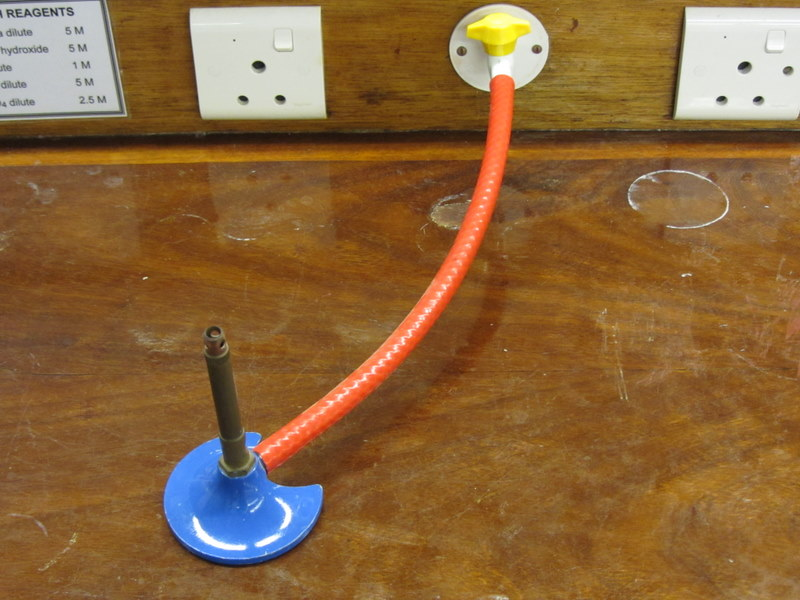
\includegraphics[width=.2\textwidth]{photos/bunsenburner.jpg} & \scalebox{.4}{\begin{pspicture}(-7.8,-1)(6.8,4)
\psset{dimen=middle,linewidth=0.053}%
% \psline[linewidth=0.05](0,5)(2,5)
% \psline[linewidth=0.04]{->}(1.7,4.5)(1,4.9)
% \uput[r](1.5,4.5){\large{toothpick with metal salt}}
\psframe(-1.25,0)(1.25,0.25)%
\psframe(-.5,1.25)(0.5,2.25)%
\multido{\n=-0.3+0.3}{3}{%
\pscircle(\n,1.75){0.1}}%
\psframe(-.25,2.25)(0.25,4.25)%
\psline(0.25,1.25)(0.25,0.5)(1.25,0.25)%
\psline(-1.25,0.25)(-.25,0.5)(-0.25,0.75)%
\psline(-2.25,0.75)(-.25,0.75)%
\psline(-2.25,1)(-.25,1)%
\psellipse(-.25,0.875)(0.1,0.125)%
\psframe[fillstyle=solid,linestyle=none](-2.25,0.75)(-0.25,1)%
\psline(-2.25,0.75)(-0.25,0.75)%
\psline(-2.25,1)(-0.25,1)(-.25,1.25)%
\pscurve(-0.25,0.5)(0,0.4)(0.25,0.5)
%flamme
\rput(0,4.25){%
\psclip{\psbezier[linestyle=none,fillstyle=gradient,gradmidpoint=0,%
gradbegin=OrangePale,gradend=yellow]%
(-0.25,0)(-0.35,0.5)(-0.4,0.75)%
(-0.35,1)(-0.25,1.5)(0.5,2)%
(0.25,1.5)(0.35,1)(0.4,0.75)%
(0.35,0.5)(0.25,0)(0,0)}%
\pspolygon[linestyle=none,fillstyle=gradient,gradmidpoint=0,gradbegin=cyan,gradend=white]%
(-0.25,0)(0.25,0)(0,1)%
\endpsclip}
\end{pspicture}} \\ \hline
Maatsilinder& \includegraphics[width=.05\textheight]{photos/Measuring_cylinder_hannesgrobe_wikimedia.jpg} & \scalebox{.4}{\begin{pspicture}(0,0)(5,5) \pstEprouvette \end{pspicture}} \\ \hline
Pipet & 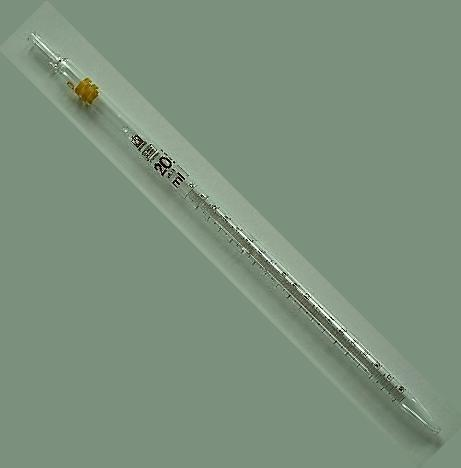
\includegraphics[width=.2\textwidth]{photos/Pipette.jpg} & \scalebox{.4}{\begin{pspicture}(0,0)(5,5) \pstpipette \end{pspicture}} \\ \hline
Horlosieglas & 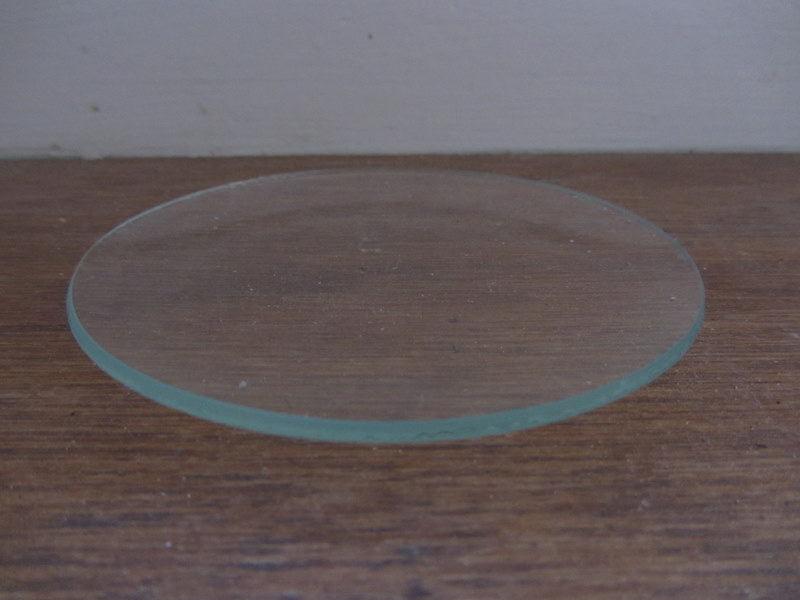
\includegraphics[width=.15\textwidth]{photos/watchglass.jpg} & \scalebox{.6} % Change this value to rescale the drawing.
{
\begin{pspicture}(0,-1.2576145)(1.8644192,-0.908)
\rput{-180.0}(2.32,0.0){\psarc[linewidth=0.04](1.16,0.0){1.16}{53.130104}{126.15819}}
\end{pspicture} 
}
 \\ \hline
% Mass meter & & \\ \hline
Termometer & \includegraphics[width=.2\textwidth]{photos/thermometer.jpg} & \scalebox{.4} % Change this value to rescale the drawing.
{
\begin{pspicture}(0,-1.74)(0.52,1.76)
\psline[linewidth=0.04cm,doubleline=true,doublesep=0.12](0.3,1.72)(0.26,-1.44)
\psline[linewidth=0.04cm](0.22,1.7)(0.38,1.7)
\psbezier[linewidth=0.04](0.2,-1.38)(0.0,-1.62)(0.5,-1.72)(0.34,-1.38)
\end{pspicture} 
} \\ \hline
Tregter & 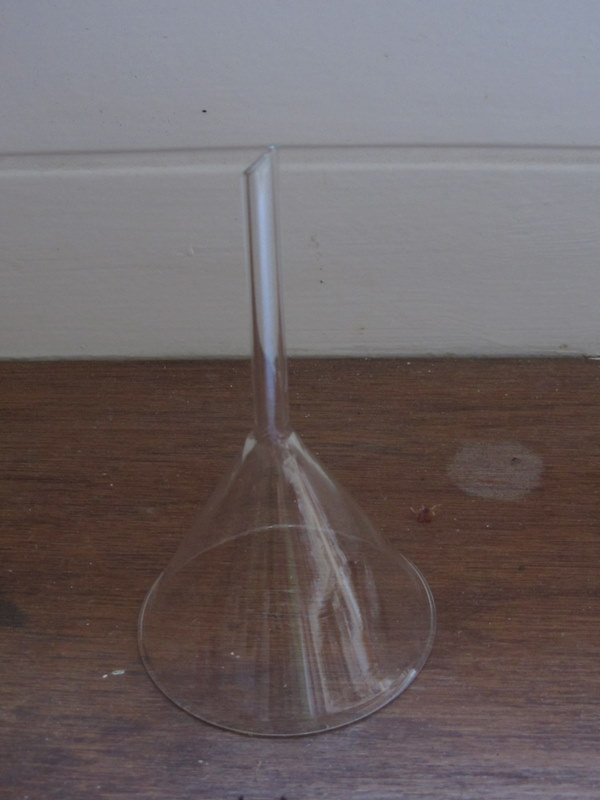
\includegraphics[width=.1\textwidth]{photos/funnel.jpg} & \scalebox{.4} % Change this value to rescale the drawing.
{
\begin{pspicture}(0,-1.17)(1.92,1.17)
\psline[linewidth=0.04cm](0.0,1.15)(0.88,0.21)
\psline[linewidth=0.04cm](1.0,0.25)(1.9,1.15)
\psline[linewidth=0.04cm,doubleline=true,doublesep=0.12](0.94,0.25)(0.94,-1.01)
\psline[linewidth=0.04cm](0.86,-0.97)(0.86,-1.15)
\end{pspicture} 
} \\ \hline
  \end{tabular} 
 \end{center}
 \end{table}

Die volgende skets wys die korrekte opstelling van die bunsenbrander om vloeistowwe te verhit:\\
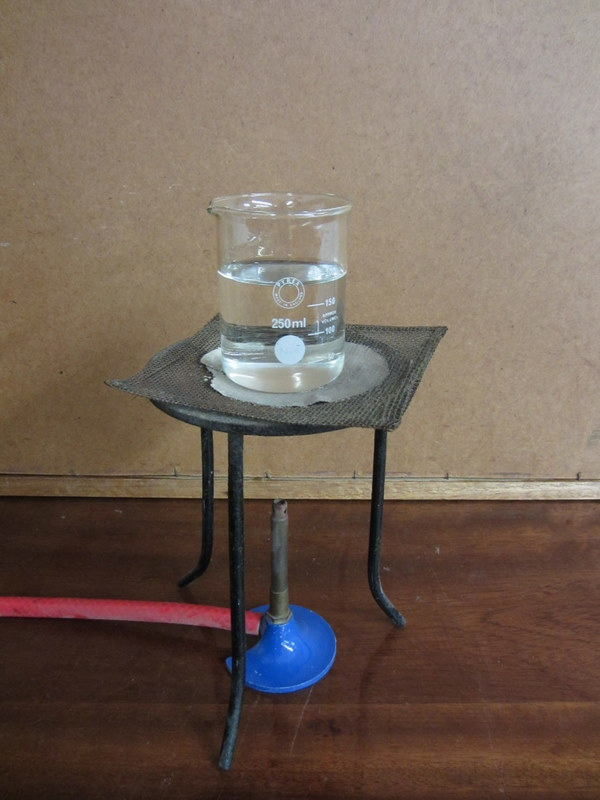
\includegraphics[width=.3\textwidth]{photos/beaker_tripod.jpg}\\
Wanneer jy enige instrument moet lees (soos  'n maatsilinder,  'n pipet ens.) moet jy seker maak dat die instrumente waterpas is en dat jou oog by die boonste vlak van die vloeistof is.

\subsection*{Algemene veiligheidsmaatreëls}
            \nopagebreak
Hier volg van die algemene riglyne en reëls wat jy moet nakom wanneer jy in  'n laboratorium werk:
\begin{enumerate}[noitemsep, label=\textbf{\arabic*}. ] 
\item Jy is verantwoordelik vir sowel jou eie as die ander mense in die laboratorium se veiligheid.
\item Moenie eet of drink in die laboratorium nie. Moet ook nie die glasware van die laboratorium gebruik om iets uit te drink nie.
\item Jy moet altyd verantwoordelik optree in  'n laboratorium. Moenie rondhardloop of grappies maak nie.
\item In geval van  'n ongeluk of waar chemikalieë gemors is, roep jou onderwyser onmiddellik.
\item Vra altyd jou onderwyser hoe om van chemiese afval ontslae te raak. Chemikalieë moet nooit in die wasbak afgegooi word nie.
\item Doen slegs die eksperimente wat jou onderwyser vir jou sê om te doen. Moet nooit sommer vir die pret chemikalieë meng nie.
\item Moet nooit eksperimente op jou eie doen nie. 
\item Kyk altyd na die inligtingstuk oor veiligheid van enige chemikalieë wat jy gaan gebruik. 
\item Volg die instruksies noukeurig. Moenie stappe verwar of in die verkeerde volgorde doen nie. 
\item Wees bewus en versigtig as jy met chemikalieë, warm glas ens. werk  
\item Maak seker dat alle bunsenbranders aan die einde van die prakties afgeskakel word en dat alle houers van chemikalieë geseël is.
\item Moet nooit water by suur voeg nie. Gooi altyd die suur by die water.
\item Moet nooit dik glasware verhit nie, dit sal breek (m.a.w. moenie maatsilinders verhit nie)
\item As jy aan chemikalieë moet ruik, sit die houer op die laboratorium werkbank en gebruik jou hande om die walms na jou toe te waai.
\item Moenie chemikalieë uit die laboratorium verwyder nie.
\item Werk altyd in  'n vertrek wat goed geventileer is. As jy eksperimente doen moet jy die vensters oopmaak.
\item Moenie bunsenbranders en vlamme onbeman los nie.
\item Moenie ruik, proe of vat aan chemikalieë tensy jy opdrag gegee word om dit te doen nie.
\item Moet nooit toetsbuise na jouself of ander mense wys nie. As jy chemikalieë verhit moet die bek van die toetsbuis altyd weg van jou en jou klasmaats gedraai wees.
\end{enumerate}
\par 
\section{Gevaartekens}
            \nopagebreak
Die tabel hieronder bevat van die mees algemene gevaartekens wat jy mag teëkom. Jy moet weet wat hierdie tekens beteken.
\begin{table}[H]
 \begin{center}
  \begin{tabular}{|l|c|p{3cm}|l|c|p{3cm}|}\hline
   \textbf{Teken} & \textbf{Simbool} & \textbf{Betekenis} & \textbf{Teken} & \textbf{Simbool} & \textbf{Betekenis} \\ \hline
\parbox[c]{4em}{
\includegraphics[width=.1\textwidth]{photos/corrosive.png}} & C & Vretend. Che\-mi\-ka\-lie\-\"e met hier\-die e\-ti\-ket kan jou vel en o\"e brand, dit brand ook gate in jou klere. Wa\-ter\-stof\-chlo\-ried of sout\-suur is 'n voor\-beeld. & \parbox[c]{4em}{
\includegraphics[width=.1\textwidth]{photos/environment.png}} & N & Om\-ge\-wings\-be\-ska\-dig\-baar. Che\-mi\-ka\-lie\-\"e  met hierdie etiket is skadelik vir die omgewing. 'n Voorbeeld is CFC's.\\ \hline 
\parbox[c]{4em}{
\includegraphics[width=.1\textwidth]{photos/explosive.png}} & E & Plofstof. Che\-mi\-ka\-lie\-\"e met hierdie etiket ontplof maklik. Loodasied is 'n voorbeeld. & \parbox[c]{4em}{\includegraphics[width=.1\textwidth]{photos/flammable.png}} & F & Ontvlambaar. Che\-mi\-ka\-lie\-\"e met  hierdie etiket vat maklik vlam. Voorbeeld: metanol \\ \hline 
\parbox[c]{4em}{\includegraphics[width=.1\textwidth]{photos/harmful.png}} & Xn & Skadelik. Che\-mi\-ka\-lie\-\"e wat so ge\"etiketeer is, word gewoonlik as skadelik vir mense aanskou.& \parbox[c]{4em}{
\includegraphics[width=.1\textwidth]{photos/irritant.png}} & Xi & Prikkelend. Che\-mi\-ka\-lie\-\"e  met hierdie etiket  ver\-oor\-saak prik\-ke\-ling van jou o\"e en vel. Voorbeeld:  wa\-ter\-stof\-pe\-rok\-sied. \\ \hline 
\parbox[c]{4em}{\includegraphics[width=.1\textwidth]{photos/oxidise.png}} & O & Oksiderend. Di\'e che\-mi\-ka\-lie\-\"e be\-vat suur\-stof wat ver\-bran\-ding van stow\-we kan ver\-oor\-saak. Ka\-li\-um\-di\-chro\-maat is 'n voorbeeld. & \parbox[c]{4em}{\includegraphics[width=.1\textwidth]{photos/toxic.png}} & T & Giftig. Che\-mi\-ka\-lie\-\"e met hierdie etiket is hoogs toksies (giftig). 'n Voorbeeld is kwik.\\ \hline 
  \end{tabular}
 \end{center}
\end{table}
\subsection*{Notas en inligting}
Jy kan al hierdie inligtingstukke oor veiligheid by \textsl{http://www.msds.com/} kry. Jy moet altyd na hierdie inligtingstukke kyk voor jy met  'n nuwe chemikalie werk. Hierdie inligtingstukke bevat inligting oor hoe om met die chemikalieë te werk en watter gevare die chemikalieë vir jou en die omgewing inhou. Jy moet altyd probeer om op  'n veilige (en die regte manier) van hierdie chemikalieë ontslae te raak. Baie chemikalieë kan nie summier in die wasbak afgespoel word nie. 

